%%%%%%%%%%%%%%%%%%%%%%%%%%%%%%%%%%%%%%%%%
% Tufte-Style Book (Minimal Template)
% LaTeX Template
% Version 1.0 (5/1/13)
%
% This template has been downloaded from:
% http://www.LaTeXTemplates.com
%
% License:
% CC BY-NC-SA 3.0 (http://creativecommons.org/licenses/by-nc-sa/3.0/)
%
% IMPORTANT NOTE:
% In addition to running BibTeX to compile the reference list from the .bib
% file, you will need to run MakeIndex to compile the index at the end of the
% document.
%
%%%%%%%%%%%%%%%%%%%%%%%%%%%%%%%%%%%%%%%%%

%----------------------------------------------------------------------------------------
%	PACKAGES AND OTHER DOCUMENT CONFIGURATIONS
%----------------------------------------------------------------------------------------

\documentclass{tufte-book} % Use the tufte-book class which in turn uses the tufte-common class

\hypersetup{colorlinks} % Comment this line if you don't wish to have colored links

\usepackage{textcomp}
\usepackage{listings} % For code highlighting
% \lstset{
%   backgroundcolor=\color[rgb]{0.98,0.98,0.98},
%   tabsize=4,
%   rulecolor=,
%   language=matlab,
%         basicstyle=\scriptsize,
%         aboveskip={1.5\baselineskip},
%         columns=fixed,
%         showstringspaces=false,
%         extendedchars=true,
%         breaklines=true,
%         prebreak = \raisebox{0ex}[0ex][0ex]{\ensuremath{\hookleftarrow}},
%         frame=single,
%         showtabs=false,
%         showspaces=false,
%         showstringspaces=false,
%         identifierstyle=\ttfamily,
%         keywordstyle=\color[rgb]{0,0,1},
%         commentstyle=\color[rgb]{0.133,0.545,0.133},
%         stringstyle=\color[rgb]{0.627,0.126,0.941},
% }

\usepackage{microtype} % Improves character and word spacing

\usepackage{lipsum} % Inserts dummy text

\usepackage{booktabs} % Better horizontal rules in tables

\usepackage{graphicx} % Needed to insert images into the document
\graphicspath{{graphics/}} % Sets the default location of pictures
\setkeys{Gin}{width=\linewidth,totalheight=\textheight,keepaspectratio} % Improves figure scaling

\usepackage{fancyvrb} % Allows customization of verbatim environments
\fvset{fontsize=\normalsize} % The font size of all verbatim text can be changed here

\newcommand{\hangp}[1]{\makebox[0pt][r]{(}#1\makebox[0pt][l]{)}} % New command to create parentheses around text in tables which take up no horizontal space - this improves column spacing
\newcommand{\hangstar}{\makebox[0pt][l]{*}} % New command to create asterisks in tables which take up no horizontal space - this improves column spacing

\usepackage{xspace} % Used for printing a trailing space better than using a tilde (~) using the \xspace command

\newcommand{\monthyear}{\ifcase\month\or January\or February\or March\or April\or May\or June\or July\or August\or September\or October\or November\or December\fi\space\number\year} % A command to print the current month and year

\newcommand{\openepigraph}[2]{ % This block sets up a command for printing an epigraph with 2 arguments - the quote and the author
\begin{fullwidth}
\sffamily\large
\begin{doublespace}
\noindent\allcaps{#1}\\ % The quote
\noindent\allcaps{#2} % The author
\end{doublespace}
\end{fullwidth}
}

\newcommand{\blankpage}{\newpage\hbox{}\thispagestyle{empty}\newpage} % Command to insert a blank page

\usepackage{makeidx} % Used to generate the index
\makeindex % Generate the index which is printed at the end of the document

%----------------------------------------------------------------------------------------
%	BOOK META-INFORMATION
%----------------------------------------------------------------------------------------

\title{AWFM Documentation} % Title of the book

\author{Alan Lewis} % Author

% \publisher{Publisher Name} % Publisher

%----------------------------------------------------------------------------------------

\begin{document}

\frontmatter

%----------------------------------------------------------------------------------------
%	EPIGRAPH
%----------------------------------------------------------------------------------------

% \thispagestyle{empty}
% \openepigraph{Quotation 1}{Author, {\itshape Source}}
% \vfill
% \openepigraph{Quotation 2}{Author}
% \vfill
% \openepigraph{Quotation 3}{Author}

%----------------------------------------------------------------------------------------

\maketitle % Print the title page

%----------------------------------------------------------------------------------------
%	COPYRIGHT PAGE
%----------------------------------------------------------------------------------------

% \newpage
% \begin{fullwidth}
% ~\vfill
% \thispagestyle{empty}
% \setlength{\parindent}{0pt}
% \setlength{\parskip}{\baselineskip}
% Copyright \copyright\ \the\year\ \thanklessauthor

% \par\smallcaps{Published by \thanklesspublisher}

% \par\smallcaps{\url{http://www.bookwebsite.com}}

% \par License information.\index{license}

% \par\textit{First printing, \monthyear}
% \end{fullwidth}

%----------------------------------------------------------------------------------------

\tableofcontents % Print the table of contents

%----------------------------------------------------------------------------------------

\listoffigures % Print a list of figures

%----------------------------------------------------------------------------------------

\listoftables % Print a list of tables

%----------------------------------------------------------------------------------------
%	DEDICATION PAGE
%----------------------------------------------------------------------------------------

% \cleardoublepage
% ~\vfill
% \begin{doublespace}
% \noindent\fontsize{18}{22}\selectfont\itshape
% \nohyphenation
% Dedicated to my family and friends.
% \end{doublespace}
% \vfill
% \vfill

%----------------------------------------------------------------------------------------
%	INTRODUCTION
%----------------------------------------------------------------------------------------

\cleardoublepage
\chapter*{Introduction} % The asterisk leaves out this chapter from the table of contents

The Analytical Well Field Model (AWFM) is a collection of computer methods for processing
large amounts of pumping and water level data at multiple wells, running analytical models,
and providing meaningful estimates aquifer and well-loss properties.

The core of AWFM provides many utilies for importing/exporting and processing data, but 
is unopinionated in that it makes it easy to add additional functionality when convenient.

With SCADA systems becoming more and more common, it is not unusual to see pumping and 
and water levels data sets containing hundreds-of-thousands or millions of records. While it is
advantageous to begin with such high-resolution data, it is largely redundant. 

\mainmatter

%----------------------------------------------------------------------------------------
% CHAPTER MATHEMATICAL BASIS
%----------------------------------------------------------------------------------------

\chapter{Mathematical Basis}

\section{Forward Model}
About forward model

\section{Inverse Model}
About inverse model

%----------------------------------------------------------------------------------------
%	CHAPTER INSTALLATION
%----------------------------------------------------------------------------------------

\chapter{Installation}

%------------------------------------------------

\section{Windows}
\lipsum[6-7]

\section{Apple}
\lipsum[6-7]

\section{Linux}
\lipsum[7-8]

%----------------------------------------------------------------------------------------
% CHAPTER: CLASSES
%----------------------------------------------------------------------------------------
\chapter{Timeseries Class}

The Timeseries class stores and processes arrays of time-value pairs. Examples of
Timeseries objects include recorded pumping rates and water levels. Internally, the
Timeseries class has separate members for holding time and value arrays, each of
which are numpy arrays.

% \begin{figure}[h]
\begin{lstlisting}[language=python]
from awfm.core import Timeseries

ts = Timeseries()
\end{lstlisting}
% \caption{Example of instantiating a Timeseries object.}
% \end{figure}

\section{append}
The \emph{append} method is used for building a Timeseries object. \emph{append}
takes two arguments, a time and a value, and appends them to the 
Timeseries object.

\begin{figure}[h]
\begin{lstlisting}[language=python]
from awfm.core import Timeseries

ts = Timeseries()
ts.append(0, 10)
ts.append(1, 12)
ts.append(2, 15)
\end{lstlisting}
\caption{Example usage of \emph{Timeseries.append}.}
\end{figure}

An important restriction to the \emph{append} method is that values
\textbf{must} be inserted in chronological order. If an attempt is made
to insert a value that is not in chronological order, \emph{append} will
simply ignore the request and log the error in Timeseries.errors.

\begin{figure}[h]
\begin{lstlisting}[language=python]
from awfm.core import Timeseries

ts = Timeseries()
ts.append(0, 10)
ts.append(1, 12)
ts.append(3, 15)
ts.append(2, 12)  # This request is not in chronological order and will be ignored.
\end{lstlisting}
\caption{Example usage of \emph{Timeseries.append} (2).}
\end{figure}


\section{zero\_below\_magnitude}

\emph{zero\_below\_magnitude} is a method that converts
any value below some user-specified magnitude to zero. 
This method is useful for dealing with SCADA systems that record
small, insignificant values while a production well is turned off. 
After running this method, the \emph{consolidate\_adjacent\_equal\_values} method
can be used to collapse a series of "off" values into one record.

\begin{figure}[h]
\begin{lstlisting}[language=python]
from awfm.core import Timeseries, io

ts = io.timeseries_from_file("my-timeseries.dat")
threshold_Q = 20 # gpm
ts_modified = ts.zero_below_magnitude(threshold_Q)
\end{lstlisting}
\caption{\emph{zero\_below\_magnitude} example script.}
\end{figure}

\begin{figure}[h]
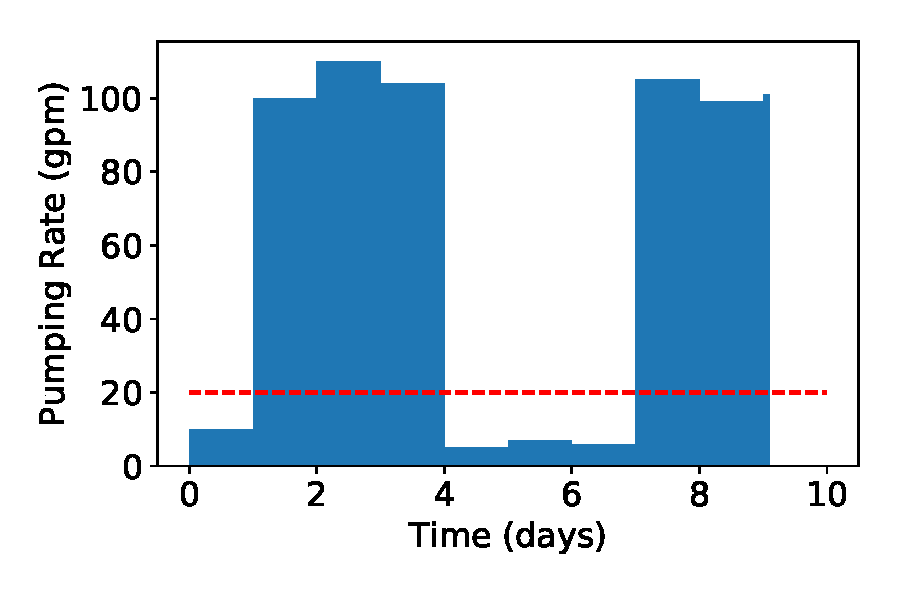
\includegraphics[width=5cm]{python/timeseries_zero_below_magnitude_before.pdf}
\hspace{\fill}
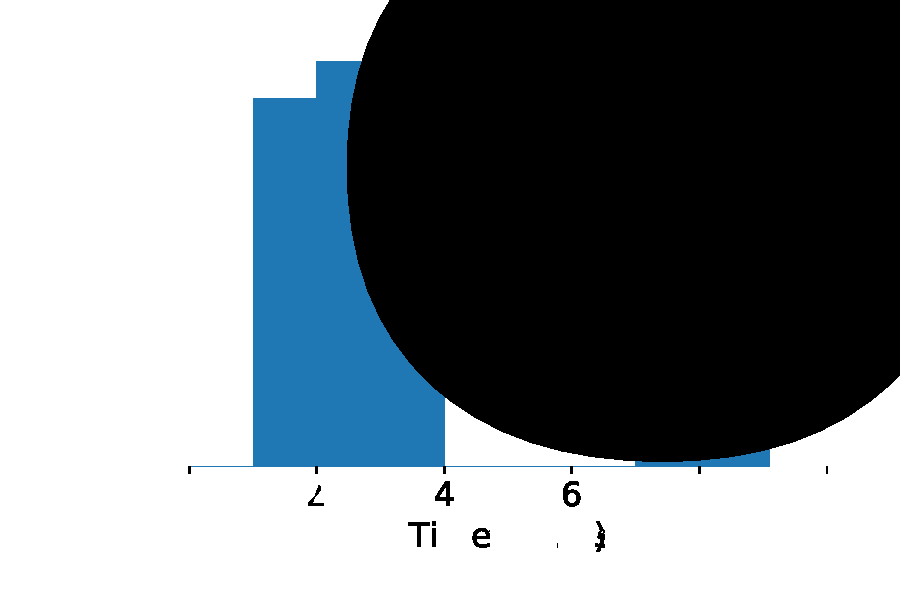
\includegraphics[width=5cm]{python/timeseries_zero_below_magnitude_after.pdf}
\caption{ \emph{zero\_below\_magnitude} example plots. 
    Original timeseries (left) is modified (right) using a threshold of 20 gpm.}
\end{figure}

\section{Well Class}
\lipsum[13-20]

\section{Dataframe Class}
\lipsum[13-20]

%----------------------------------------------------------------------------------------
% CHAPTER EXAMPLES
%----------------------------------------------------------------------------------------
\chapter{Examples}

\section{Example: Reducing Timeseries Data}

\section{Example: Simple Forward Model}
\lipsum[13-20]

\section{Example: Custom Dataframe}
\lipsum[13-20]

%----------------------------------------------------------------------------------------

\backmatter

%----------------------------------------------------------------------------------------
%	BIBLIOGRAPHY
%----------------------------------------------------------------------------------------

\bibliography{bibliography} % Use the bibliography.bib file for the bibliography
\bibliographystyle{plainnat} % Use the plainnat style of referencing

%----------------------------------------------------------------------------------------

\printindex % Print the index at the very end of the document

\end{document}